% CS 454/554 Midterm Mini-Project — Technical Report
% Build: latexmk -pdf main.tex   (Overleaf: compiler pdfLaTeX, main document main.tex; bibliography via BibTeX, style unsrt)
%
% Overleaf is linked to the whole GitHub repository through GitHub Sync (Menu → GitHub).
% In Overleaf, edit ONLY files under docs/report/. Pull from GitHub before editing; push when you stop.
% CI compiles this file on every push and publishes the PDF as the "report-pdf" workflow artifact.
%
% Ownership convention for collaboration:
%   Sections 1–4 and the appendix: drafted by Claude from the evidence files; the student revises.
%   Sections 5 and 6: written by the student; Claude edits for length and traceability.
% Word budgets (hard, from the handout): §1–§4 together ≈ 800–1,100; §5 = 500–750; §6 = 200–300.
% Count with:  texcount -inc -sum main.tex   (or Overleaf → Menu → Word Count)

\documentclass[11pt,letterpaper]{article}
\usepackage[margin=1in]{geometry}
\usepackage[T1]{fontenc}
\usepackage[utf8]{inputenc}
\usepackage[expansion=false]{microtype}
\usepackage{graphicx}
\usepackage{booktabs}
\usepackage{xcolor}
\usepackage{hyperref}
\hypersetup{colorlinks=true,linkcolor=black,citecolor=blue!50!black,urlcolor=blue!50!black}
\usepackage{enumitem}
\setlist{nosep}

% Evidence citation: \evid{file}{section} → (evidence/file, section)
\newcommand{\evid}[2]{\textsf{\footnotesize(evidence/#1, #2)}}
\newcommand{\code}[1]{\texttt{#1}}

\title{One Service, Two Deployment Environments\\
\large CS 454/554 Midterm Mini-Project --- Technical Report}
\author{CS 454/554 --- Introduction to Cloud Computing, Fall 2026 (graduate section)}
\date{October 2026 \quad\textbullet\quad Repository: \url{https://github.com/RemyMartinRosenhoover/CS-554-MidTerm}}

\begin{document}
\maketitle

\section{Deployment overview}

The project runs one small HTTP service in two environments and records how each manages it. Everything sits in four layers (Figure~\ref{fig:topology}). The physical host is a Windows 11 workstation running VMware Workstation 17.6.1. Inside it, a virtual machine named \code{cs554-vm} runs Ubuntu Server 24.04.5 with 2 vCPUs, 4 GiB of RAM, and a 25 GiB disk, attached to VMware's NAT network \code{192.168.197.0/24}; the host owns \code{.1} on that network and the VM received \code{.134} from VMware's DHCP \evid{00-host-vm.md}{VM facts}. Inside the VM, Docker Engine 29.1.3 runs the containers. For Part~2, Docker Compose 2.40.3 runs the service container directly. For Part~3, a k3d 5.9.0 cluster runs a single k3s 1.37.1 node as a Docker container on the same engine, and the Kubernetes Pods run inside that node container. At the bottom of every path is the same application process: Node 22 executing the course starter's \code{server.js}, which answers \code{GET /} with a JSON body (service name, message, hostname, and a request counter kept in process memory) and \code{GET /health} with HTTP 200.

Both environments use one container image, built once inside the VM from \code{app/Dockerfile}. Compose runs it from the local Docker image store; the cluster receives it through \code{k3d image import}, and the Deployment sets \code{imagePullPolicy: Never} so the cluster can only use the imported image \evid{02-kubernetes.md}{Import the same application image}. No registry is involved. The image was first built as \code{cs554-midterm:1.0}; the CS~554 readiness experiment added a four-line readiness toggle to \code{/health} and rebuilt as \code{1.1}, which both environments now run. Earlier captures that show \code{1.0} are unchanged and historical.

\begin{figure}[htbp]
  \centering
  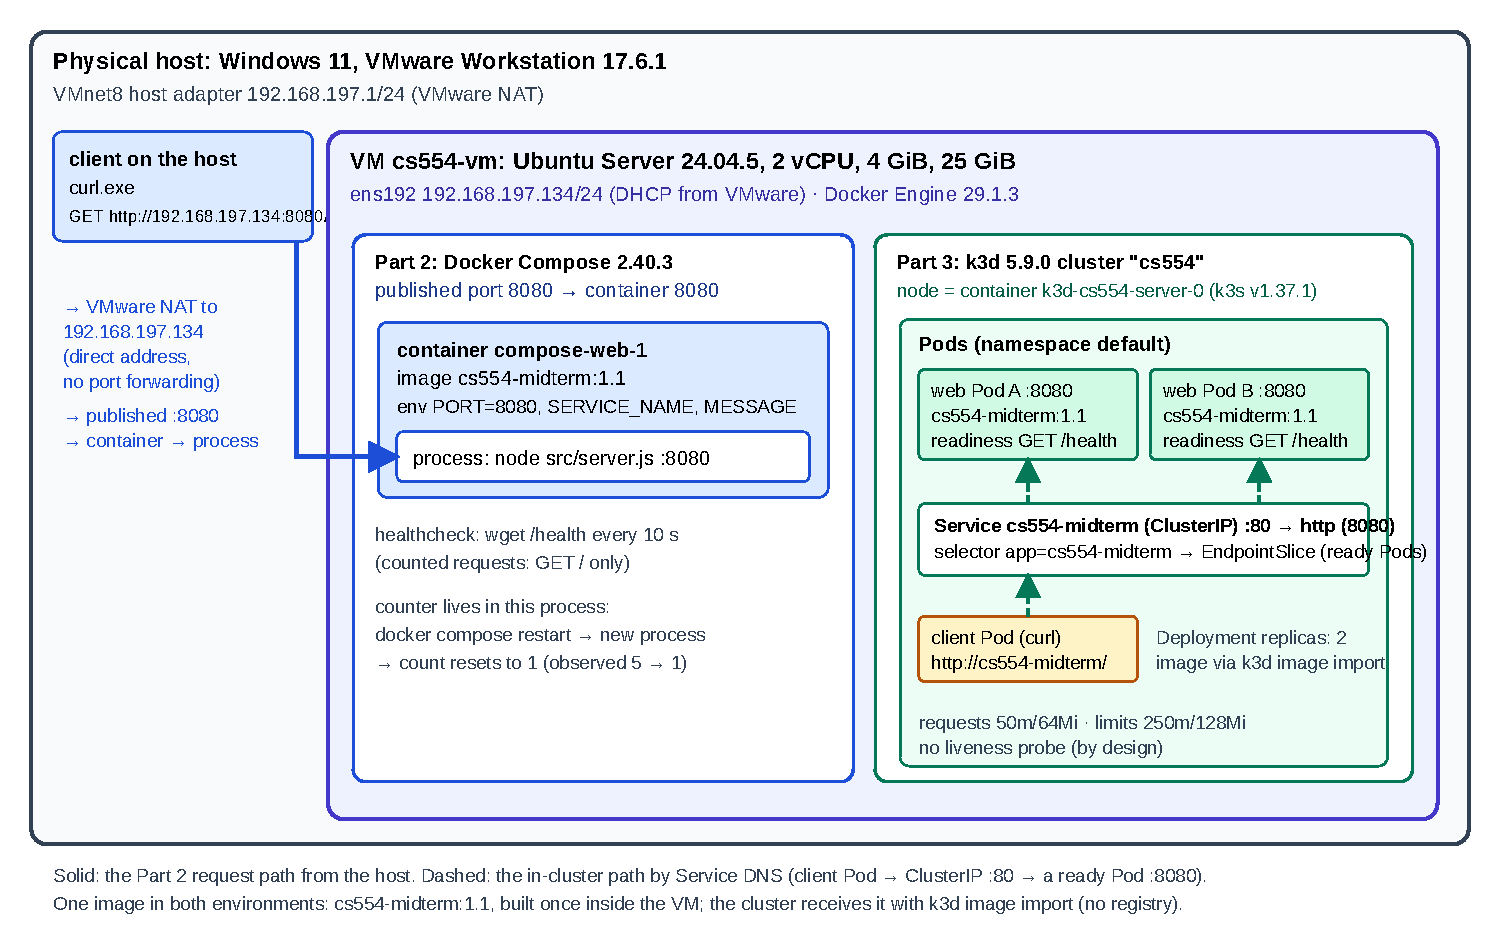
\includegraphics[width=\textwidth]{figures/diagram.pdf}
  \caption{Host, VM, container, and application layers, with the Part~2 request path from the host (solid) and the in-cluster Kubernetes path (dashed). Ports and addresses are labeled as observed.}
  \label{fig:topology}
\end{figure}

\section{Docker Compose inside the VM}

The Compose file declares one service, \code{web}, built from \code{../app}, configured entirely through environment variables (\code{PORT}, \code{SERVICE\_NAME}, \code{MESSAGE}) read from an uncommitted \code{.env} file whose defaults are committed as \code{.env.example}, with VM port 8080 published to the container's port 8080 and a health check that calls \code{/health} every ten seconds \evid{01-compose.md}{Resolved Compose configuration}. The health check deliberately targets \code{/health}, which the service does not count, so it never disturbs the request counter.

From inside the VM, three requests to \code{GET /} returned counts 1, 2, and 3 from the container hostname \code{864d1c1b9d87}, and \code{/health} returned HTTP 200 \evid{01-compose.md}{VM requests and health}. From the Windows host, \code{curl.exe http://192.168.197.134:8080/} returned count 4 from the same container \evid{01-compose.md}{Windows host request}. The host reaches the VM directly on its NAT address; VMware's NAT device routes between the host adapter and the guest, so no port forwarding was configured. \code{docker compose ps} showed the container \code{Up (healthy)}, and the logs showed the startup line \code{Listening on port 8080} followed by one JSON line per request, including the periodic \code{/health} probes \evid{01-compose.md}{Startup and request logs}.

The restart experiment is the observation the rest of the report leans on. With the count at 5, \code{docker compose restart} stopped and started the container: the logs recorded \code{Received SIGTERM; stopping.} and then a fresh \code{Listening on port 8080}, and the next request returned count 1 \evid{01-compose.md}{Restart and counter reset}. The container kept its name and hostname; only the process inside it was new, and the counter lived in that process. A failed health check in Compose would have marked the container unhealthy but would not by itself have restarted it. \code{docker compose down} removed the container and its network; the service was then brought back up for the walkthrough \evid{01-compose.md}{Cleanup demonstration}.

\section{Kubernetes}

The cluster runs inside the same VM: k3d creates the node as a Docker container from the image \code{rancher/k3s:v1.37.1-k3s1}, pinned so that the server matches the installed kubectl 1.37.1 \evid{02-kubernetes.md}{Create the cluster}. A Deployment named \code{cs554-midterm} asks for two replicas of the image, labels its Pods \code{app=cs554-midterm}, and a ClusterIP Service of the same name selects that label and maps port 80 to the container's named port \code{http} (8080). After \code{kubectl apply}, the Deployment reported \code{2/2}, both Pods were \code{1/1 Running}, and the Service's EndpointSlice listed two endpoints \evid{02-kubernetes.md}{Apply and two ready replicas}.

Requests were sent through the Service in two ways, because they demonstrate different things. From a client Pod inside the cluster, six requests to \code{http://cs554-midterm/} by DNS name were answered by both Pods, each with its own counter; this shows the Service resolving to ready backends across replicas, though not round-robin ordering or fairness \evid{02-kubernetes.md}{In-cluster Service requests}. A \code{kubectl port-forward svc/cs554-midterm 18080:80} session inside the VM answered three requests all from one Pod: port-forward uses the Service's selector only to choose a Pod, then tunnels to that Pod through the API server, so it proves reachability but says nothing about traffic distribution \evid{02-kubernetes.md}{VM-local Service port-forward}.

Deleting one Pod produced the behavior that distinguishes Kubernetes from Compose. With Pods \code{mkspb} and \code{ndjs4} running, \code{kubectl delete pod} on \code{mkspb} was followed within three seconds by a new Pod, \code{2jmll}, in \code{ContainerCreating}, which was \code{Running} at three seconds and \code{1/1} ready at six; the ReplicaSet returned to desired/current/ready 2 and logged a \code{SuccessfulCreate} event \evid{02-kubernetes.md}{Automatic Pod replacement}. Kubernetes replaced the Pod because the ReplicaSet controller continuously reconciles the Pods it observes against the Deployment's declared \code{replicas: 2}; one Pod short, it created another, without any further command. The replacement's first request counted 1 \evid{02-kubernetes.md}{Replacement process counter}. The comparison with Part~2 is direct: Compose restarted the same container's process because an operator told it to, whereas Kubernetes created a different Pod, with a new name, on its own. Both lost the in-memory counter, because in both cases the process was new; what differed was who decided and what identity survived.

\section{Controlled troubleshooting: the Service selector}

A Service is a label query, and the EndpointSlice is the result of that query. The experiment changed one line in \code{service.yaml}, the selector from \code{app: cs554-midterm} to \code{app: cs554-midterm-typo}, and applied it; nothing else changed \evid{03-selector-break.md}{Exact selector change}. From the client Pod, three requests to the Service by DNS name failed with \code{curl: (7) Failed to connect to cs554-midterm port 80 ... Could not connect to server}, exit code 7. A port-forward session started fresh after the change exited with \code{error: timed out waiting for the condition}, and its request also failed with exit 7 \evid{03-selector-break.md}{In-cluster client symptoms; Fresh port-forward failure}. The session had to be fresh: an old port-forward would have stayed pinned to the Pod it chose earlier and hidden the fault.

The observations separate the cause from everything it was not. Both Pods stayed \code{1/1 Running} with zero restarts and their labels unchanged; the Deployment's UID, generation, and spec were byte-identical before, during, and after; the Service's selector read \code{app=cs554-midterm-typo}; the EndpointSlice had no endpoints (kubectl 1.37 renders an empty endpoint set as \code{<unset>} and a blank \code{Endpoints:} line, where older versions printed \code{<none>}); and the Pods' logs from the moment of the change onward contained only readiness probes and not one \code{GET /} \evid{03-selector-break.md}{Failure diagnosis}. The cause follows: no Pod carried the label the selector asked for, so the EndpointSlice controller computed an empty backend set, kube-proxy had no destination for Service traffic, and port-forward could not pick a Pod. Re-applying the correct \code{service.yaml} restored two endpoints, and both client paths succeeded again, with the same Pod names and zero restarts throughout \evid{03-selector-break.md}{Correct selector and recovery}.

Healthy Pods therefore prove nothing about reachability through a Service. Readiness is a statement about a process: it can serve. A Service's endpoints are a statement about a match: these Pods carry the labels this selector names. The two are evaluated independently, and either can be true while the other is false. A diagnosis that stops at \code{kubectl get pods} sees two healthy replicas and no problem; it must also compare the selector to the labels, inspect the EndpointSlice, and test a client path that depends on the match.

\section{OpenStack deployment analysis}
% STUDENT-AUTHORED. Target 500–750 words across §5.1–§5.5 and the closing comparison (table excluded).
% Course material: Exercise 05 README and OPENSTACK-SETTINGS.md in the course repository (cite as \cite{ex05,ex05settings}).
% Concrete class names: profile devstack, region RegionOne, image ubuntu-24.04, flavor m1.small,
%   network private / subnet private-subnet, router router1, external network public,
%   floating IP from public, security group default + rules, student key pair, cloud-init user data.

\subsection{Resources and choices}
% Table of resource · value · created by me / supplied by the admin, then prose:
% justify the modest flavor from our own numbers (free -h: 505 MiB used of 3.8 GiB with the service running);
% whether persistent block storage is needed (the counter is deliberately in-process; the image rebuilds from the repo).

\begin{table}[h]
\centering\small
\begin{tabular}{@{}lll@{}}
\toprule
Resource & Value in the class cloud & Who provides it \\
\midrule
Image & \code{ubuntu-24.04} & administrator \\
Flavor & \code{m1.small} & administrator (I choose it) \\
Key pair & my own, created once & me \\
Tenant network / subnet & \code{private} / \code{private-subnet} & administrator \\
Router to external network & \code{router1} $\rightarrow$ \code{public} & administrator \\
Security group & \code{default} + my rules & me (rules) \\
Floating IP & allocated from \code{public} & me \\
User data & cloud-init: install Docker, run Compose & me \\
\bottomrule
\end{tabular}
\caption{OpenStack resources for the workload, following the class environment \cite{ex05settings}.}
\end{table}

% TODO (student): prose for §5.1.

\subsection{Service responsibilities}
% Keystone (authenticate the CLI via the devstack profile; scope to the project), Glance (store/serve the image),
% Nova (schedule and boot the instance from image + flavor; inject key pair and user data),
% Neutron (port on private, router1 to public, floating IP mapping, security-group rules).
% Where Compose fits: cloud-init user data installs Docker + Compose and runs `docker compose up -d` from the repo,
% exactly as our VM build did, so the instance converges with no login. Cinder: not proposed; say when it would be.
% TODO (student).

\subsection{Request path}
% External client → floating IP on public → router1 NAT to the instance's private address → security group on the port
% evaluates the rule → VM kernel → Docker published 8080 → container → Node process.
% Name the rule (ingress TCP 8080) and distinguish it from TCP 22 (SSH, operators only) and ICMP (ping, diagnostic, optional).
% Security groups are stateful: no egress rule needed for the reply.
% TODO (student).

\subsection{Failure analysis}
% Instance ACTIVE, client cannot reach the service. Layered checks with the evidence collected at each:
% (1) on the instance: docker compose ps, curl localhost:8080/health, container logs  → app/container layer
% (2) VM network: ip addr, ss -ltnp (8080 bound on 0.0.0.0), host firewall                → VM layer
% (3) cloud network: server show (addresses), floating ip list (association), security group rule list, router show
% (4) client: curl -v to the floating IP; ping if ICMP allowed.  Say which layer "refused" vs "timeout" vs "404" points to.
% TODO (student).

\subsection{Operational complexity}
% Running OpenStack = Keystone, Glance, Nova, Neutron + databases, message queue, agents on every compute node,
% so that a user can run one `server create`. One example from the class demonstration or troubleshooting discussion
% (your own memory of class is best; fallback: the course's DevStack notes say a rebuild beats repairing a broken install,
% and the restricted-network appendix shows a TLS-intercepting proxy breaking image pulls inside cloud VMs).
% Distinguish an infrastructure setup problem (stops every tenant; the operator fixes it) from an application deployment
% problem (one project; the user fixes it).
% TODO (student).

\subsection{Closing comparison}
% When a VM with Compose is sufficient; what Kubernetes added in our experiment (declared replica count enforced,
% automatic replacement, readiness-based traffic exclusion, a Service abstraction a selector can silently break).
% TODO (student).

\section{CS 554 extension: resource settings and the readiness experiment}
% STUDENT-AUTHORED. Target 200–300 words.
% Settings: requests 50m/64Mi, limits 250m/128Mi (QoS Burstable). Request = what the scheduler reserves; limit = the ceiling
% enforced at run time (CPU throttled; memory → OOM kill). Why these numbers: the service is one Node process; the VM
% showed 505 MiB used in total with it running; 250m leaves burst headroom without one replica starving the other on 2 vCPUs.
% Readiness vs restart: the probe governs endpoint membership. In the experiment Pod A went 0/1 Running with 0 restarts,
% its counter continued 4 → 5 → 6 across failure and recovery, and all in-cluster traffic went to B
% (evidence/04-readiness-554.md). A liveness failure or restart would have produced a new process and a reset counter.
% Why this method: a running Pod's probe is immutable, so the documented application toggle (READINESS_FILE) was the
% permitted route; the template changed only in the pre-experiment rollout; the experiment touched one file in one Pod.
% TODO (student).

\bibliographystyle{unsrt}
\bibliography{references}

\end{document}
